\subsection{Description/materials}
%Describe the concept, layer structure and the materials used for the firewall. Show how the low resistance Control System ground connection is achieved.

We are using standard concept of firewall as described in the rules (T4.5.4). So the firewall is made from 2 layers. The first one is 0,5 mm thick aluminum sheet and the second one is 0,8 mm thick glass fiber/polyester plastic sheet with UL 94-V0 certificate (type: UPM 203 / UPM 71/S included in appendix). These are glued together and bended to the shape of final firewall. Aluminum sheet is oriented to the dangerous side and glass fiber to the driver side.
\subsubsection{Position in car}
%Provide CAD-renderings showing all relevant parts. Mark the parts in the rendering, if necessary.

Firewalls are located behind the seat and above the front motor controller (under drivers knees). These firewalls are connected with "firewall tunnel" where are located the high voltage cables.

\begin{figure}[H]
	\centering
	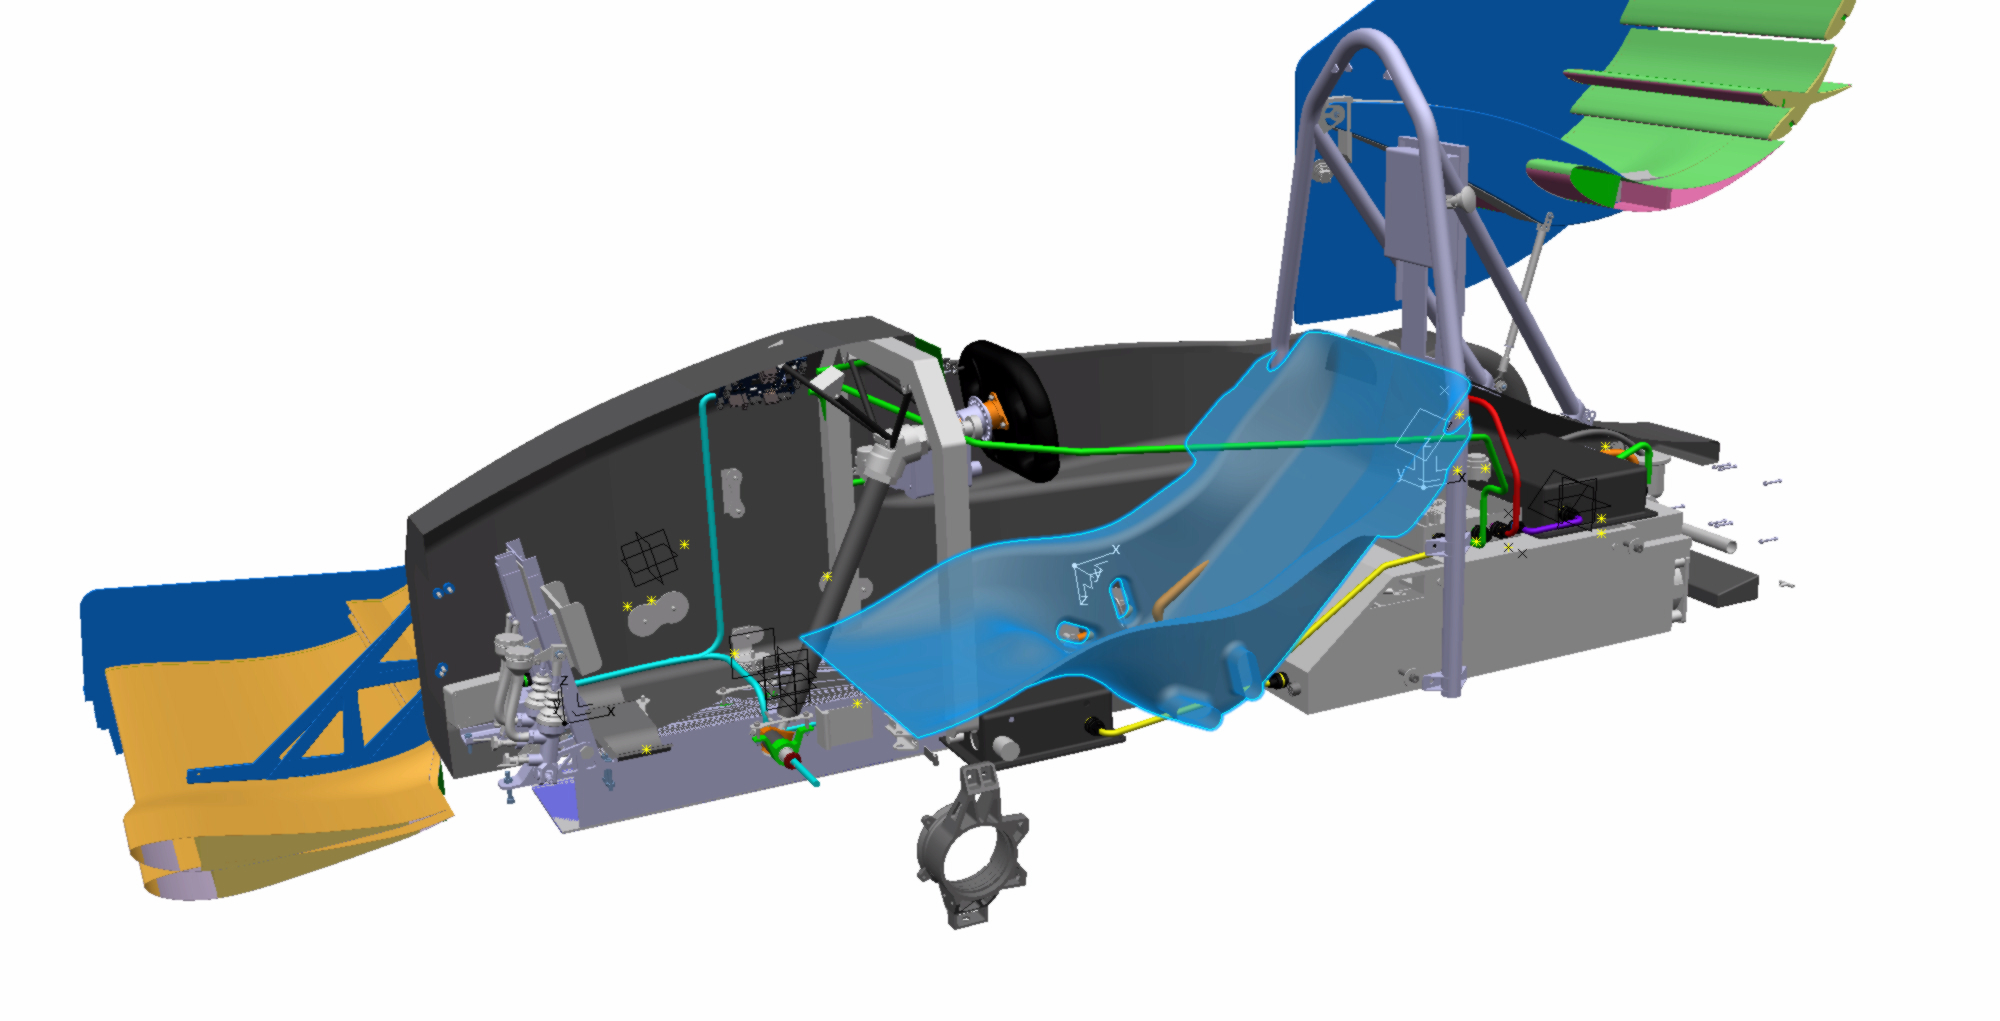
\includegraphics[width=\textwidth]{./img/Firewall-position.jpg}
	\caption{Firewall position.}
	\label{fig:Firewall-position}
\end{figure}